\documentclass[a4paper, 12pt]{article}

\input{"$HOME/Desktop/Studia/LaTeX/setup.tex"}

\title{\textsc{Generatory liczb pseudolosowych - rozkłady skorelowane w 2D}\\ - sprawozdanie}
\author{Wojciech Orłowski}
\date{\today}

\begin{document}
    \maketitle

    \section{Wstęp}

    Celem ćwiczenia jest zapoznanie studenta z generowaniem liczb pseudolosowych o danym rozkładzie dwuwymiarowym.
    Rozkłady te będą skorelowane (rozkłady po transformacji) i nieskorelowane (rozkład normalny).
    \\
    \\
    Rozkład normalny zostanie wygenerowany za pomocą metody Boxa-Mullera.
    Metoda ta polega na zamianie zmiennych z układu kartezjańskiego na zmienne biegunowe.
    Następnie w tym układzie jesteśmy w stanie obliczyć dystrybuantę i skorzystać z metody odwracania dystrybuanty.
    Ostateczny wzór na parę zmiennych o rozkładzie normalnym w 2D ma postać
    \[ X = \sqrt{-2 \ln(1 - U_1)}\cos(2\pi U_2), \]  
    \[ Y = \sqrt{-2 \ln(1 - U_1)}\sin(2\pi U_2), \]
    gdzie $U_1, U_2$ oznaczają zmienne wylosowane o rozkładzie normalnym.
    \\
    \\
    Następnie zmienne wylosowane w ten sposób są normalizowane.
    Ich odległość od układu wspólłrzędnych ma wynosić 1.
    Zostało to wykonane w celu uzyskania rozkładu jednorodnego na okręgu
    \[ X' = \frac{X}{\sqrt{X^2 + Y^2}},\]
    \[ Y' = \frac{Y}{\sqrt{X^2 + Y^2}}.\] 
    Za pomocą pary zmiennych $X', Y'$ tworzymy rozkład jednorodny w kole, odpowiednio je skalując.
    W tym celu skorzystamy z kolejnej zmiennej losowej, będącej pierwiastkiem z liczby o rozkładzie jednorodnym $U(0,1)$.
    \[ R = \sqrt{U}\] 
    \[ X'' = RX' \]
    \[ Y'' = RY' \]
    W kolejnym etapie zajęć została wykonana transformacja algebraiczna, zamieniająca rozkłady kuliste na rozkłady elipsoidalne.
    W transformacji tej korzystamy z macierzy obrotu oraz odpowiedniego skalowania.

    \section{Wyniki}

    \subsection*{Rozkład normalny}

    Wygenerowany za pomocą metody Boxa-M\"ullera zestaw liczb \{$X_i, Y_i$\} można nanieść na wykres (wykres \ref{fig:box_mul}).
    
    \begin{figure}[h]
        \centering
        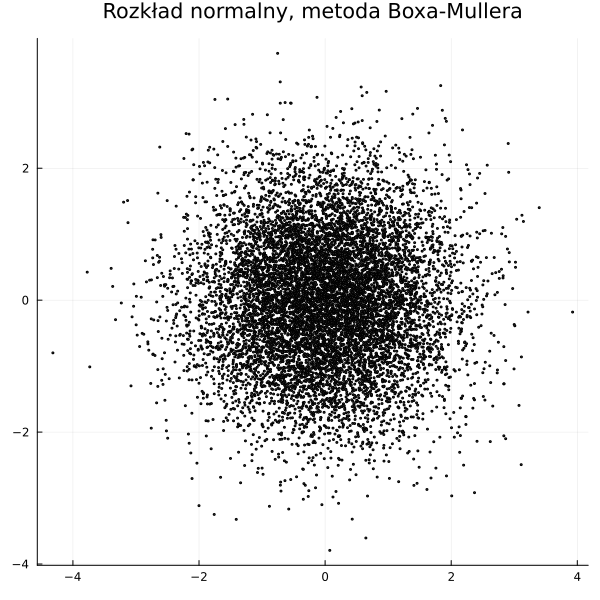
\includegraphics[width=0.6\textwidth]{"../galeria/box_muller.png"}
        \caption{Pary liczb \{$X_i, Y_i$\} wygenerowane metodą Boxa-M\"ullera, $N=1\text{e}4$ wygenerowanych liczb.}
        \label{fig:box_mul}
    \end{figure}

    \noaka Punkty przedstawione na rys. \ref{fig:box_mul} przypominają rozkład normalny dwuwymiarowy.
    Bez wykonania jednak testów statystycznych ciężko sprawdzić dokładnośc wygenerowanych liczb.
    Warto też dodać, że wygenerowany zestaw liczb reprezentuje rozkład $N(0,1)$, czyli mający wartość oczekiwaną w (0,0), a odchylenie standardowe równe jest 1.  

    \newpage

    \subsection*{Rozkład jednorodny w kole}

    Dokonując operacji przedstawionych w wstępie normalizujemy odległość punktów od środka układu wspólłrzędnych. 
    W kolejnym etapie losowo skalujemy punkty, tak że uzyskujemy rozkład jednorodny w środku koła jednostkowego.
    \begin{figure}[H]
        \centering
        \begin{subfigure}{0.45\textwidth}
            \centering
            \includegraphics[width=\textwidth]{"../galeria/na_kole.png"}
            \caption{}
        \end{subfigure}
        \begin{subfigure}{0.45\textwidth}
            \centering
            \includegraphics[width=\textwidth]{"../galeria/w_kole.png"}
            \caption{}
        \end{subfigure}
        \caption{Wygenerowane pary liczb \{$X_i,Y_i$\} o rozkładzie jednorodnym (a) na kole, (b)  w kole.}
        \label{kolo}
    \end{figure}   

    \noaka Ponownie dokonując analizy jakościowej (rys. \ref{kolo}) można stwierdzić, że udało się wygenerować liczby w kole o rozkładzie jednorodnym.
    Jednak generowanie w ten sposób liczb o rozkładzie jednorodnym na kole może się wydawać nieefektowne.
    Wystarczyłoby wylosować liczbę o rozkładzie jednorodnym z przedziału kątowego (od $0$ do $2\pi$).
    Ta liczba i tak jest losowana w sposób jednorodny podczas losowania kąta w metodzie Boxa-M\"ullera.

    \subsection*{Rozkład jednorodny w elipsie}

    Dokonując transformacji punktów wylosowanych wcześniej (rys. \ref{kolo} (b)) przekształcany jest rozkład jednorodny w kole na rozkład jednorodny w elipsie (rys. \ref{elipsa_jednorodny}).

    \begin{figure}[H]
        \centering
        \includegraphics[width=0.4\textwidth]{"../galeria/elipsa_jednorodny.png"}
        \caption{Pary liczb \{$X_i, Y_i$\} uzyskane poprzez obrót i skalowanie liczb wylosowanych w kole.}
        \label{elipsa_jednorodny}
    \end{figure}

    \noaka Elipsa przedstawiona na rys. \ref{elipsa_jednorodny} została wykonana poprzez obrócenie punktów wygenerowanych na kole o kąt $\pi/4$, które wcześniej zostały odpowiednio przeskalowane.
    Można już zauważyć, że występuję pewna korelacja między punktami.
    Jeżeli $X$ jest duże, to $Y$ też jest raczej duże, natomiast gdy $X$ jest małe $Y$ też jest małe.
    Taką zależność można zmierzyć współczynnikiem korelacji, który w tym przypadku wynosi 0.9214.
    
    \subsection*{Transformacja rozkładu normalnego}

    Podobnej transformacji możemy wykonać na zestawie danych o rozkładzie normalnym przedstawionym na rys. \ref{fig:box_mul}.
    \begin{figure}[H]
        \centering
        \includegraphics[width=0.6\textwidth]{"../galeria/elipsa_normalny.png"}
        \caption{Pary liczb \{$X_i, Y_i$\} uzyskane poprzez transformacje par o rozkładzie normalnym.}
        \label{elipsa_normalny}
    \end{figure}

    \noaka Tym razem można znaleźć punkt, który jest dalej od centrum elipsy, jednak jednocześnie w jej centrum jest dużo większe zagęszczenie.
    Ponownie można zauważyć wysoką korelacje między zmiennymi $X_i$ i $Y_i$. 
    Tym razem możemy porównać także analityczne rozważania dotyczące korelacji tych zmiennych.
    Według rozważań analitycznych, macierz kowariancji dla rozkładu normalnego po transformacji daje się zapisać jako
    \[ \Sigma = AA^T, \]
    gdzie $A$ to macierz transformacji.
    Za pomocą tej macierzy jesteśmy w stanie obliczyć współczynnik korelacji, który wyniósł 0.9231.
    Natomiast licząc ten sam współczynnik z estymatorów dla wylosowanej próbki otrzymano 0.9235. 
    Te dwie wartości są sobie bardzo bliskie.
    Może to być sposobem walidacji metody generowania liczb pseudolosowych.

    \newpage

    \section{Podsumowanie}

    Podczas ćwiczenia udało się wygenerować liczby o zadanym rozkładzie w dwóch wymiarach.
    Sprawdzono także korelacje między wygenerowanymi zestawami.
    Już dla niskiej ilości wylosowanych liczb wartości korelacji są bliskie do teoretycznych.
    

\end{document}
